\subsubsection{Low-Temperature Geochemistry and Astrobiology}
\index{Bau, Michael}

\paragraph{Research Team}
Michael Bau (Professor), Brian Alexander (PhD student), Serkan
Kulaksiz (PhD student), Jule Mawick (lab technician), Thomas
Schirmer
(Post-doc) \\


Low-temperature processes operating at the Earth's surface not only
affect the atmosphere-hydrosphere system but also the upper
lithosphere and the biosphere. The chemical composition of seawater,
river water, and groundwater and of precipitates from such waters are
controlled by these processes that, therefore, are of major interest
in \textit{applied geosciences} such as \textit{environmental
geochemistry} and \textit{ore deposit research}.

The chemical evolution of the Earth's surface systems
throughout 4 billion years of geological record and their interaction
with the evolving biosphere are recorded in chemical sediments. Hence,
chemical sediments have become one of the focus areas of
\textit{astrobiology} which ultimately studies the possibilities for
(maybe exstinct) life on other planets and moons.

Hence, the trace element (and isotope) geochemistry of natural
waters and chemical sediments is a research focus of geochemistry at
IUB.

\paragraph{Highlights}
In the field of applied environmental geochemistry significant advance
has been made in 2006 in the study of the behaviour of anthropogenic
gadolinium (Gd) in rivers in northwestern Germany, in the Weser
Estuary and in the southern North Sea. All major rivers in
northwestern Germany display large positive Gd anomalies that indicate
the presence of anthropogenic Gd derived from contrast agents used in
magnetic resonance imaging. This mi\-cro\-pol\-lu\-tant cannot be removed by
common sewage treatment technology and enters rivers with the clear
water discharge from waste water treatment plants. As elsewhere, the
natural rare earths and yttrium (REY) are particle-reactive elements
that in the Weser River water associate with the colloidal
load. Therefore, the REY are removed from the dissolved REY pool as
these colloids aggregate in the low-salinity part of the Weser
Estuary. In the mid- and high-salinity part, the REY are remobilized
from particles and transferred from the particulate back into the
dissolved REY pool. These processes cause characteristic fractionation
across the REY series, eventually leading to low La/Lu ratios,
positive La anomalies, and super-chondritic Y/Ho ratios of the
riverine REY input into seawater. In marked contrast to the natural
REY, the anthropogenic Gd behaves conservatively and transits through the
Weser Estuary almost unaffected. This indicates that the speciation of
anthropogenic Gd is different from that of natural Gd and suggests a
long environmental half-life of the anthropogenic Gd complexes used as
contrast agents. We found an anthropogenic Gd anomaly in the
southwestern North Sea, off the coast of the East Frisian Islands,
where it is likely to result from input of anthropogenic Gd from the
rivers Rhine, Ems, and probably Thames. The widespread distribution of
anthropogenic Gd is an example of how the increasing use of formerly
``exotic'' (ultra)trace elements in high-tech processes will in the
future significantly hamper studies of the distribution and
geochemical behaviour of such elements in natural systems.

Future studies in collaboration with the water authorities in
the State of Bremen will focus on the quantification of the annual Gd
flux from the waster water treatment plant at Bremen-Seehausen into
the Weser River and on the attempt to trace its inflow into the Baltic
Sea. In collaboration with A. Koschinsky (IUB) and A. K\"ohler (Alfred
Wegener Institute, Bremerhaven), we started to investigate wether or
not anthropogenic Gd enters the food chain, using blue mussels as
sample organisms. We also started projects (funded by Bundesanstalt
Geowissenschaften Rohstoffe, Hannover) looking into the distribution
of and evaluating the economic importance of high-tech elements (Se,
Te, Nb, Ta, Zr, Hf, Ge, Y, REE) in Mn nodules.

Activities related to astrobiology continued to focus on Meso- and
Neoarchean sequences in South Africa and Canada. With our partners in
the University of Johannesburg we do a detailed study of the trace
element distribution and the neodymium (Nd) isotopic composition of
shales and banded iron-formation (BIF) in the 2,900 Ma old Pongola
Supergroup. Both, the REY distribution and the Nd isotope ratios,
suggest that in marked contrast to BIFs elsewhere, the iron and the
REY deposited in the shallow-water Moozan Formation of the Pongola
Supergroup did not originate from seafloor basalts from which they had
been mobilized by high-temperature hydrothermal fluids, but from upper
crustal sources from which they had been mobilized either by rivers or
by porewaters. It further appears that in spite of intense
syn-depositional alteration of some of the shale layers intercalated
with the BIF, their Th-U ratios have not been changed, suggesting that
this alteration occurred in an anoxic environment. This is fully
compatible with the absence of any Ce anomaly from the REY patterns of
the BIFs and is further evidence for anoxic conditions even in very
shallow surface seawater 2,900 Ma ago.

These studies are currently extended to include chemical sediments
deposited between 2,600 and 2,400 Ma ago and focus on trace elements
and, in collaboration with A. Eisenhauer (Inst. f. Meeresforsch.,
Geomar Kiel), on Ca isotopes.

\begin{figure}[ht]
  \begin{center}
    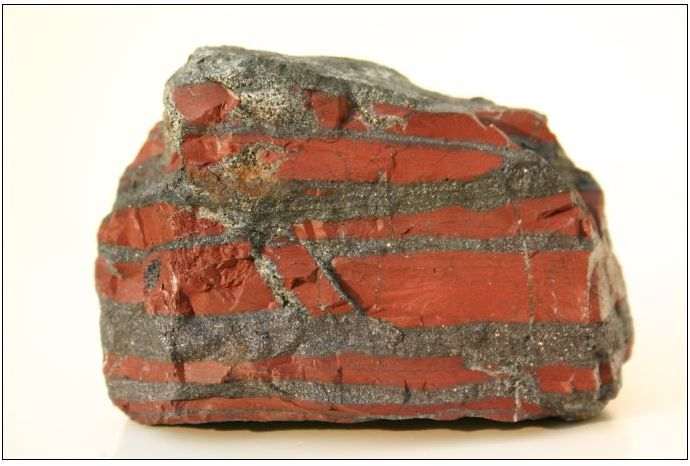
\includegraphics[width=6cm]{GeoAstro/Bau/Slide1.png}
    \mycaption{2,700 million years old banded iron-formation from the
Temagami Greenstonebelt, Ontario, Canada. Alternating
bands of iron-oxides and iron-rich quartz, that accumulated at the
floor of the Archean  ocean and preserved the trace
element and Nd isotopic composition of contemporaneous seawater}
\label{fig:bau}
   \end{center}
\end{figure}


\paragraph{Organization}
% list the (research) events you have organized, if any,

\begin{enumerate}
\item Organizer of the workshop: \textit{``Banded Iron-Formations: A
Precambrian Enigma''} 19. -- 22.10.2006 at International University
Bremen funded by European Science Foundation, ESF

\item Chair of German - South African Exchange Program between International
University Bremen, Germany, and University of Johannesburg, South
Africa

\item Elected Chairman of the Geochemistry Division and board member of the
Deutsche Mineralogische Gesellschaft, DMG (German Mineralogical
Society)

\item ``Examinateur''  and international committee member at l'Universite de Rennes I, France, for O. Pourret: ``\textit{Impact de la matiere organique sur le comportement des terres rares en solution: etude experimentale et modelisation''}.

\item Convener of Symposium on ``Early Earth and Astrobiology'' at the
Annual Meeting of the DMG at Hannover, Germany

\end{enumerate}

\paragraph{Collaborations}
\noindent

Regional:
\begin{enumerate}
\item {\sl International University Bremen}\\ Prof. Dr. A. Koschinsky
\item {\sl Alfred Wegener Institut, Bremerhaven}\\ Prof. Dr. A. K\"ohler
\item {\sl Inst. f. Meeresforschung Geomar, Kiel}\\ Prof. Dr. A. Eisenhauer
\item {\sl Universit\"at Kiel}\\ Prof. Dr. D. Garbe-Sch\"onberg
\item {\sl  Universit\"at Hannover}\\ Prof. Dr. F. v. Blanckenburg
\end{enumerate}

National:
\begin{enumerate}
\item {\sl GeoForschungsZentrum Potsdam}\\ Prof. Dr. P. Dulski, Prof. Dr. P. M\"oller, Prof. Dr. V. L\"uders
\item {\sl Universit\"at Bonn}\\ Prof. Dr. C. M\"unker
\item {\sl Humboldt Universit\"at Berlin}\\Prof. Dr. U. Riller
\item {\sl Universit\"at T\"ubingen}\\ Prof. Dr. A. Kappler
\end{enumerate}

International:
\begin{enumerate}
\item {\sl Natural History Museum, Stockholm, Sweden} \\Prof. Dr. P. Andersson
\item {\sl University of Leeds, U.K.}\\Prof. Dr. D. Banks
\item {\sl University of Johannesburg, South Africa}\\ Prof. Dr.J. Gutzmer,
N. Beukes
\item {\sl United States Geological Survey, Menlo Park, USA}\\ J. Hein
\item {\sl Laurentian University, Sudbury, Canada}\\Prof. Dr. B. Kamber
\end{enumerate}


\paragraph{Grants}
% list the running grants in 2005, if none have been received, please delete this
% subsection.
\begin{enumerate}
\item Funding:  DFG \\
Project: \emph{redoxabh\"angige Fraktionierung von Selen und Tellur
in geochemischen Systemen},  KO 2906/4-1 (IUB Project no. 50161)
P.I.: A. Koschinsky, M. Bau \\
Duration: October 2003 - September 2006

\item {Bundesanstalt f\"ur Geowissenschaften und Rohstoffe Hannover,
BGR} ``Literaturstudie Manganknollen'' IUB project no. 50166 P.I.:
A. Koschinsky, M. Bau


\item {European Science Foundation, ESF} Workshop ``Banded
Iron-Formations: A Precambrian Enigma'' Organizer: M. Bau
\end{enumerate}

\nocite{Bau1,Bau2,Bau3}
